\textbf{Problem 44. (a) (b)} \\
\hrule 

A result called \textbf{Chebyshev's inequality} states that for any probability distribution of an rv X and any number k that is at least 1, $P(|Xi\mu| \geq k\sigma) \leq \frac{1}{k^2}$. In words, the probability that the value of X lies at least k standard deviation from its mean is at most $\frac{1}{k^2}$.

\textbf{a. What is the value of the upper bound for k = 2, 3, 4, 5 and 10?}

\textbf{b. Compute $\mu$ and $\sigma$ for the distribution of Exercise 13. Then evaluate $P(|Xi\mu| \geq k\sigma)$ for the values of k given in part (a). What does this suggest about the upper bound relative to the corresponding probability?}

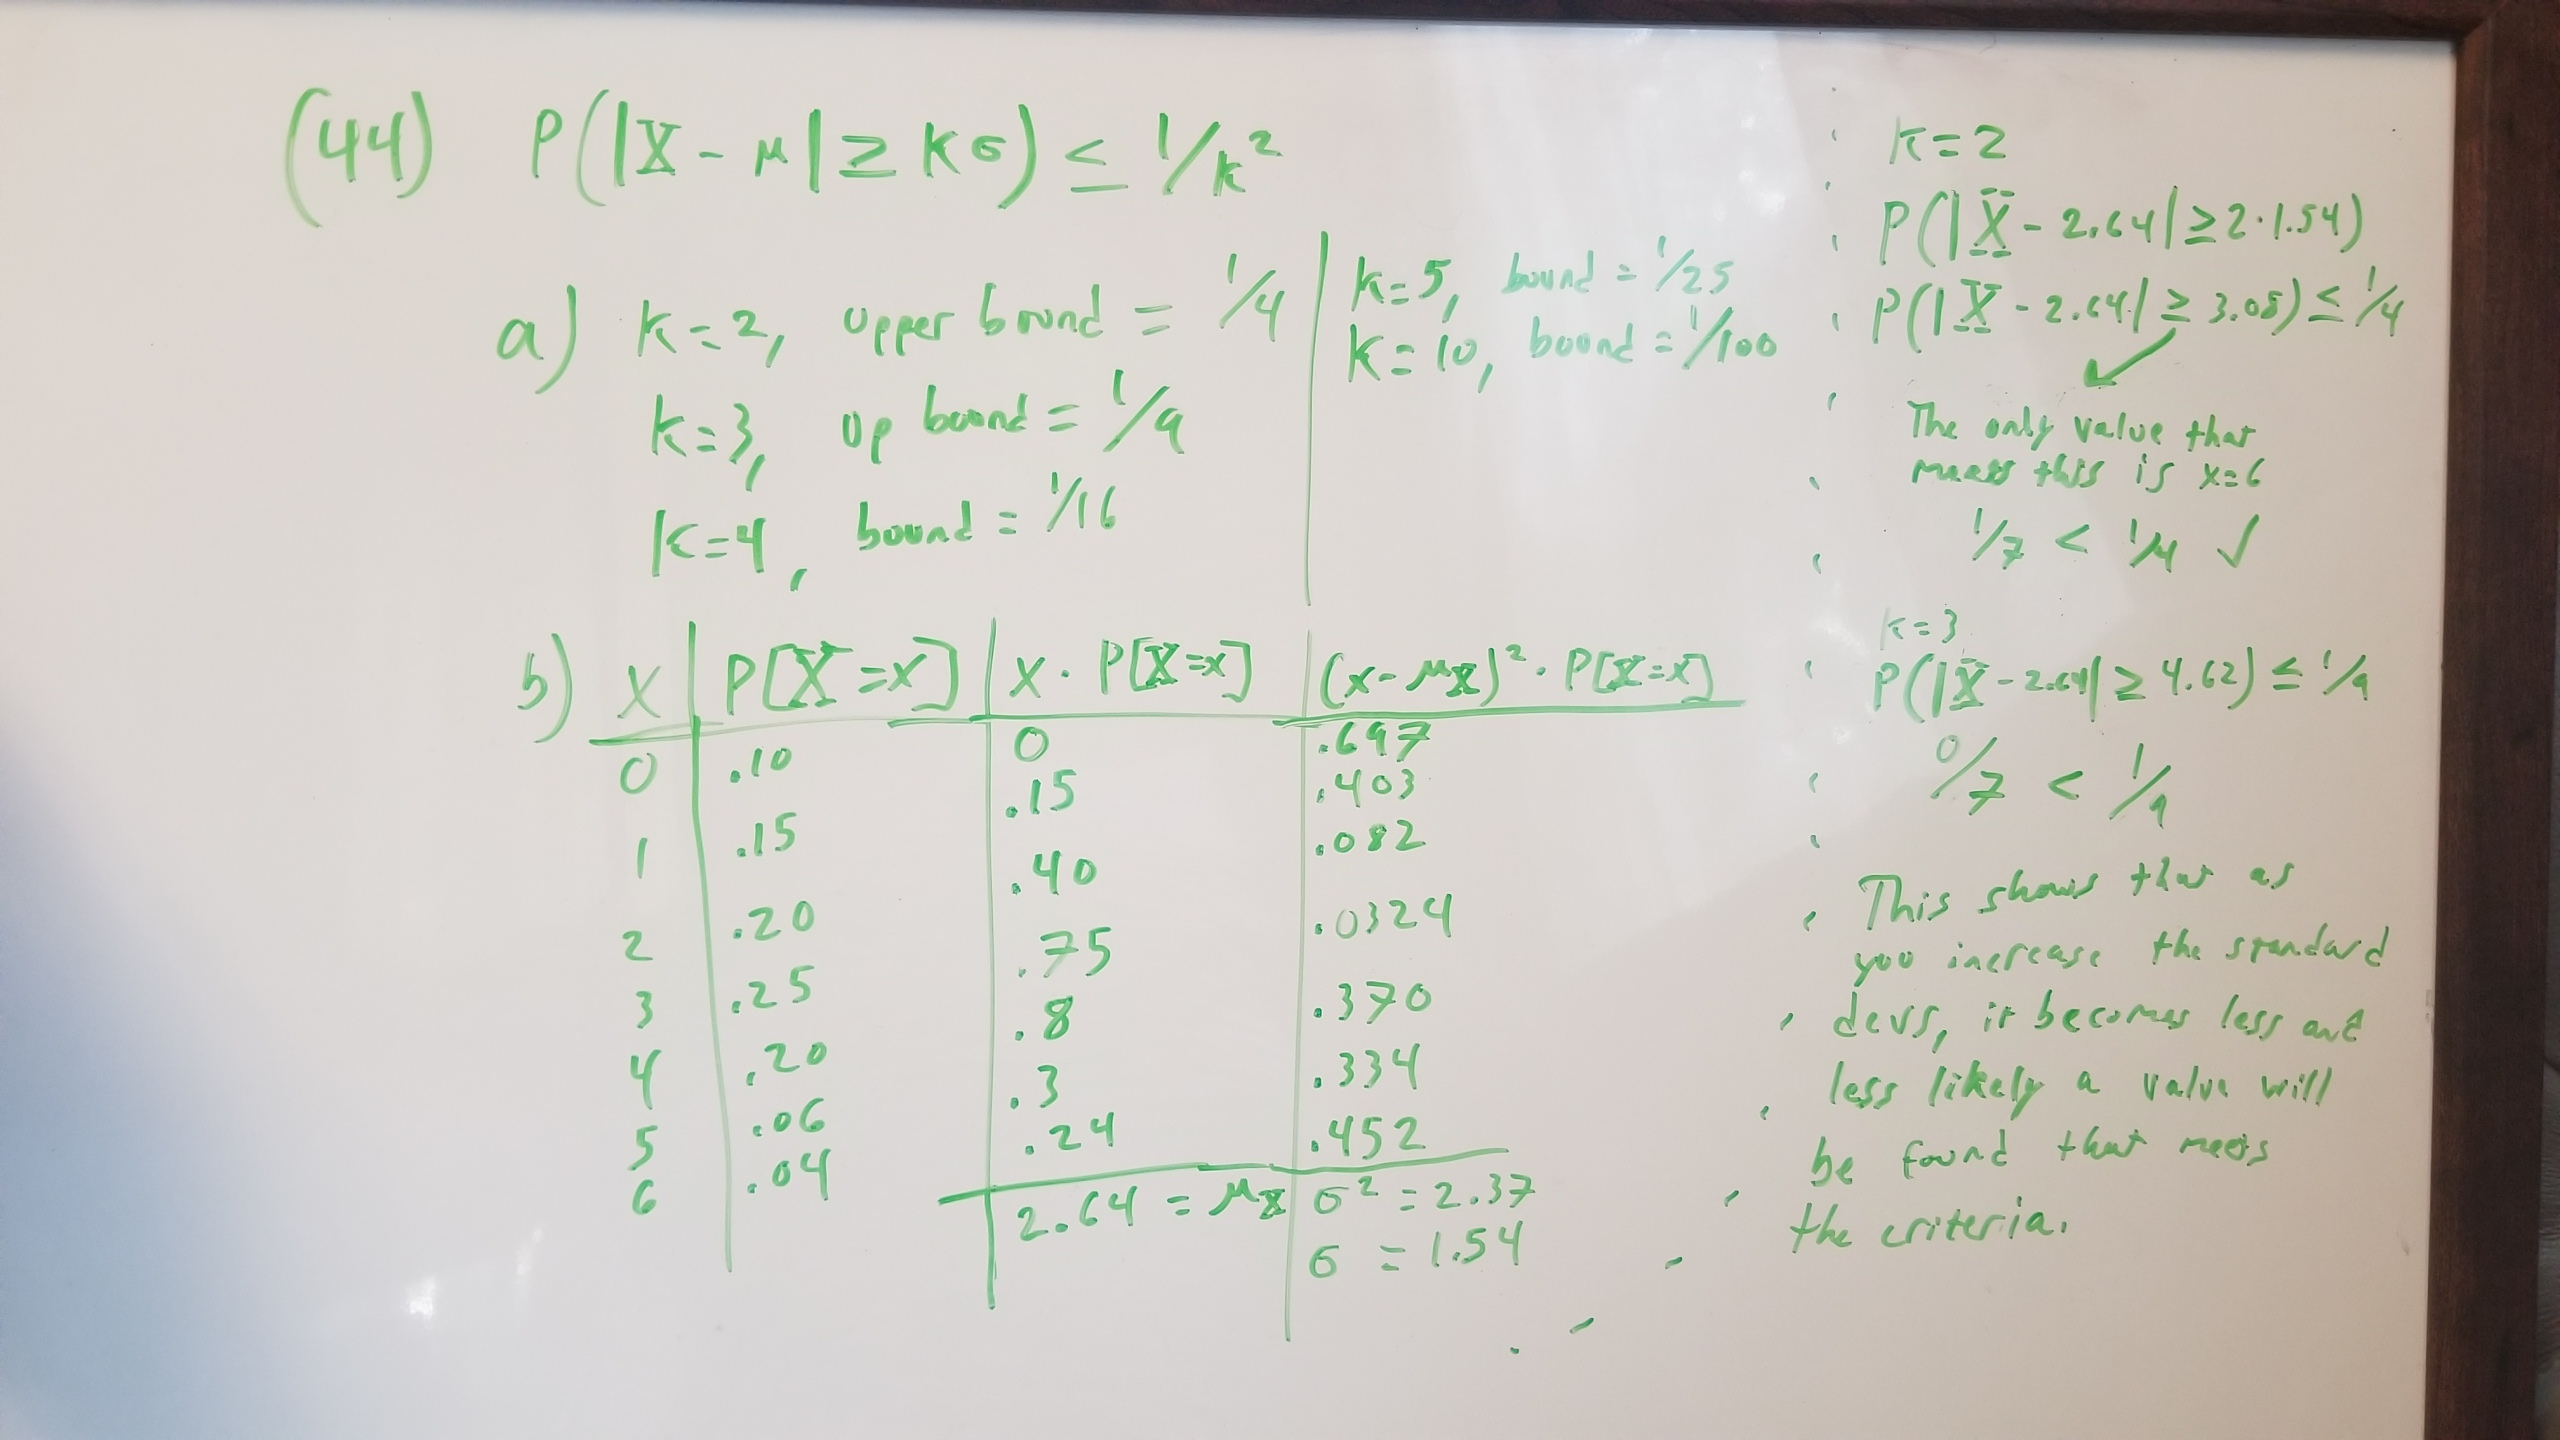
\includegraphics[scale=.2]{images/whw4/3.3.44.jpg}